\chapter{Machine Learning Theory} \label{chap:ml}

This section will act as a theory section for the machine learning models used. A machine learning models are a subset of artificial intelligence models. Machine learning models extract rules from data, which can then be applied to classify, or estimate components of another dataset called the \textit{target variable}. What makes mahine learning models different from other artificial intelligence models, is that the rules for making predictions on the target variable are not given to the model explicitly. Instead, the models are given data and extract the rules for making predictions themselves. Machine learning algorithms are formally divided into \textit{supervised learning}, \textit{unsupervised learning} and \textit{semi-supervised learning}. Supervised learning models require labelled datasets to extract information from the dataset, and are usually used to perform classification tasks, or to estimate a variable that is considered dependent on the input variables (regression). Unsupervised learning algorithms do not require labelled datasets. There also exist hybrid models called \textit{semi-supervised learning} that use a combination of labelled and unlabelled datasets. The two sections of this chapter are dedicated to the two most central machine learning models encountered in this work; clustering and \acrshort{ann}. The clustering section will give the theoretical background of the similarity measures, and clustering algorithm used, and the deep neural networks section will DO SOMETHING. In the paragraph below the definition of a time series is given, which is the definition that is used throughout this work. \bigskip

\subsection*{What Is a Time Series?}
A time series is defined as a set of observations $\{x_t\}$ recorded at a specific time $t$. A discrete time series is a time series where the set of times when observations are made ($T_0$) is discrete \cite{brockwell_davis_advanced}. A multivariate time series can be viewed as a set of vectors $\{\mathbf{x}_t\}$ where each set of vector elements $\{x^i_t\}$ is an individual time series. This means that the elements of the same vector $[x^1_t, x^2_t,...,x^N_t]$ are separate observations. A \acrshort{gls} curve extracted from an ultrasound video from the \acrshort{4ch} view of a patient can be considered a univariate time series, while the \acrshort{gls} curves extracted from the ultrasound videos of all the three views for a single patient can be considered a multivariate time series. \bigskip

\section{Clustering}
There are three types of \acrshort{tsc}, \textit{whole-series \acrshort{tsc}}, \textit{subsequence \acrshort{tsc}} and \textit{time-point \acrshort{tsc}}. Whole-series \acrshort{tsc} is when multiple ''whole'' time series are clustered with respect to each other. Subsequence \acrshort{tsc} comprises the clustering of subsequences of the same time series with respect to each other. The defining difference between whole-series and subsequence \acrshort{tsc} is that whole-series \acrshort{tsc} clusters multiple time series while subsequence \acrshort{tsc} clusters different subsequences of the same time series. When performing time-point \acrshort{tsc} the goal is to cluster individual observations of a time series with regard to to each other. In this review we will only consider work using whole-series \acrshort{tsc}, so when the phrase \textit{time-series clustering} is used, one can assume that whole-series \acrshort{tsc} is what is being refered to. \bigskip

Whole series \acrshort{tsc} can broadly be divided into three main approaches. The raw-data based approach, the feature-based approach and the model based approach. In the raw-data based approach one measures the similarity between the raw time series themselves and clusters them based on this. When clustering raw time series the majority of the work goes into selection of similarity metric and clustering algorithm, and one clusters the time series with regard to similarity in time or similarity in shape \cite{tsc_rev}. In the feature-based approach one also clusters time series with regard to similarity in time, and shape, but the work is somewhat shifted away from choice of similarity metric and over to choice of representation. Either to extract more relevant information from the time series, or to reduce the computational complexity of the similarity measurement. In the model-based approach the goal is most often to cluster time series with regard to the underlying data generating process \cite{moar_mpl_tsc}. The underlying assumption being that two time series that appear different might still have been generated by the same process.

\begin{figure}
    \begin{center}
    \tikzstyle{int} = [pin edge={to-,thin,black}]
\tikzstyle{sqr}  = [rectangle, rounded corners, minimum width=4.25cm, minimum height=1cm,text centered, draw=black, fill=white]
\tikzstyle{arrow} = [thin,->,>=stealth]

\begin{tikzpicture}[node distance=1.75cm]

%% Model-based approach
\node (inp_mod) [int] {Raw time series};
\node (rep_mod) [sqr, below of=inp_mod] {Model parameters};
\node (sim_mod) [sqr, below of=rep_mod] {Similarity measurement};
\node (clu_mod) [sqr, below of=sim_mod] {Clustering};
\node (out_mod) [int, below of=clu_mod] {Cluster assignments};

%% Feature-based approach
\node (inp_fea) [int, right of=inp_mod, xshift=3cm] {Raw time series};
\node (rep_fea) [sqr, below of=inp_fea] {Extracted features};
\node (sim_fea) [sqr, below of=rep_fea] {Similarity measurement};
\node (clu_fea) [sqr, below of=sim_fea] {Clustering};
\node (out_fea) [int, below of=clu_fea] {Clusters assignments};

%% Raw-data based approach
\node (inp_raw) [int, right of=inp_fea, xshift=3cm] {Raw time series};
\node (sim_raw) [sqr, right of=sim_fea, xshift=3cm] {Similarity measurement};
\node (clu_raw) [sqr, below of=sim_raw] {Clustering};
\node (out_raw) [int, below of=clu_raw] {Clusters assignments};

%% Names
\node (nam_mod) [int, below of=out_mod, yshift=1cm] {\textbf{(Model-based)}};
\node (nam_fea) [int, below of=out_fea, yshift=1cm] {\textbf{(Feature-based)}};
\node (nam_raw) [int, below of=out_raw, yshift=1cm] {\textbf{(Raw-data based)}};

%% Arrows
\draw [arrow] (inp_mod) -- (rep_mod);
\draw [arrow] (rep_mod) -- (sim_mod);
\draw [arrow] (sim_mod) -- (clu_mod);
\draw [arrow] (clu_mod) -- (out_mod);

\draw [arrow] (inp_fea) -- (rep_fea);
\draw [arrow] (rep_fea) -- (sim_fea);
\draw [arrow] (sim_fea) -- (clu_fea);
\draw [arrow] (clu_fea) -- (out_fea);

\draw [arrow] (inp_raw) -- (sim_raw);
\draw [arrow] (sim_raw) -- (clu_raw);
\draw [arrow] (clu_raw) -- (out_raw);
\end{tikzpicture}
    \end{center}
    \caption{Illustration of the three approaches to whole-series \acrshort{tsc}, and their components. The illustration is inspired by figure 2 in \textcite{tsc_rev}.}
    \label{fig:tsc_approaches}
\end{figure}

The common denominator of the three approaches to \acrshort{tsc} mentioned is that they are all made up of three distinct parts: representation method, similarity measurement and clustering algorithm. This is illustrated in figure \ref{fig:tsc_approaches}. Another key aspect of the \acrshort{tsc} model is what the \textbf{objective} is. There are broadly regarded to be three objectives, one can cluster with regard to: Similarity in time, similarity in shape and similarity in change CITATION. When calculating the similarity between all combinations of time series, the resulting similarity metric are stored in what is called a \textit{dissimilarity matrix}. The choice of similarity metric is important in a raw-data approach as it decides which aspects of the time series will be used to measure (dis)similarity, and has a has a significant impact on the time-complexity of the clustering system. \acrshort{pvc} has a similar approach as raw-data based \acrshort{tsc}, the dissimilarity between data points are measured which are passed on the clustering algorithm. In the subsection below, the dissimilarity measures used in the clustering models of this work are described.

\subsection{Dissimilarity metric}
When clustering point-values, the choice of metric used to measure dissimilarity between the data objects are usually some sort of distance measure. The choices of distance measures are varied and plentiful. Options include: Euclidean distance, Manhatten distance and Minkowski distance. In the \acrshort{pvc} models the Euclidean distance is used because it is the most easy to interpret geometrically. It is defined in equation \eqref{eq:ed} for two data objects $x$, and $y$ of $N$ dimensions.

\begin{equation}
    ED(x,y) = \sqrt{\sum_{i = 1}^N (x_i - y_i)^2}
    \label{eq:ed}
\end{equation}

\begin{figure}
    \centering
    \begin{subfigure}[b]{0.49\textwidth}
        \centering
        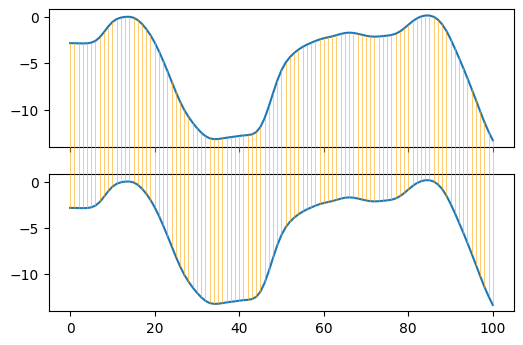
\includegraphics[width=0.99\textwidth]{machine-learning/warping_lines_1_curve.png}
        \caption{Sample-wise Euclidean distance.}
        \label{fig:ed_ex}
    \end{subfigure}
    \begin{subfigure}[b]{0.49\textwidth}
        \centering
        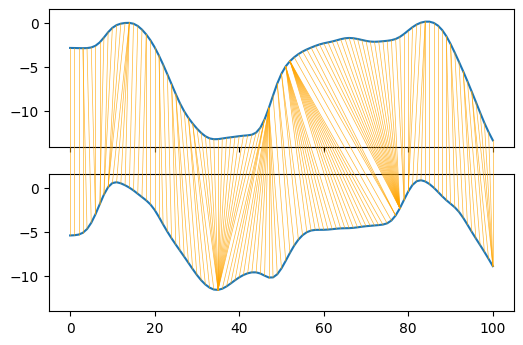
\includegraphics[width=0.99\textwidth]{machine-learning/warping_lines_2_curves.png}
        \caption{\acrshort{dtw} distance.}
        \label{fig:dtw_ex}
    \end{subfigure}
    \caption{An illustration of the difference between sample-wise Euclidean distance between time series, and \acrshort{dtw} distance between time series.}
    \label{fig:ed_dtw_ex}
\end{figure}

In the raw-data based approach to \acrshort{tsc}, choice of dissimilarity metric is paramount, and is chosen based on what objective of the \acrshort{tsc} is, and the different lengths of the time series to be compared. When clustering with regard to similarity in shape, the similarity metric can be lock-step (one-to-one) or elastic (one-to-many) \cite{tsc_rev}. An example of a lock-step measure is the use of Euclidean distance to measure the distance between time series sample-wise. However, this becomes problematic when the time series are not of equal length. \acrfull{dtw} distance is a powerful alternative for Euclidean distance to measure the shape-based distance between two time series. To understand how the \acrshort{dtw} distance works as a dissimilarity metric, one can imagine that it warps one time series such that the two series are equal in length, and then measures the Euclidean distance between them. This is illustrated in figure \ref{fig:ed_dtw_ex}. \acrshort{dtw} is probably most famous from speech recognition where it is applied to find out which phoneme\footnote{Phoneme is a term from speech recognition, and refers to the biggest unit of sound for which the frequency spectrum is constant. phonemes are considered as the ''atomic sounds'' that make up speech.} in a dictionary of phonemes is the optimal fit to a recorded sound. To calculate the \acrshort{dtw} distance between two time series $x$ and $y$ of length $n$ and $m$ respectively. First an $(n \times m)$ matrix is constructed called the \acrfull{lcm}. Element $\mathrm{LCM}(i,j)$ is the sample-wise quadratic distance between $x_i$ and $y_i$ ($(x_i - y_i)^2$). The next step is to create a warping path $P = \{p_1, p_2, ..., p_L\}$ across the \acrshort{lcm}. The warping path must fulfill three conditions: the boundary condition, the continuity condition and the monotonicity condition. 

\begin{enumerate} 
    \item \textbf{Boundary}: The path must begin, and end in the corners of the \acrshort{lcm}. $p_0 = \mathrm{LCM(1,1)}$, $p_L = \mathrm{LCM(n,m)}$ 
    \item \textbf{Continuity}: Two adjacent warping steps $p_k$ and $p_{k+1}$ must be equal to adjacent elements on the \acrshort{lcm}. This means that the matrix elements $p_k$ and $p_{k+1}$ are equal to must be adjacent horizontally, vertically or diagonally.
    \item \textbf{Monotonicity}: The warping path must increase monotonically. This means that the warping path cannot go backwards index-wise. If one combines the continuity, and monotonicity constraints, and lets $p_k = \mathrm{LCM}(i,j)$, valid values for $p_k$ are $\mathrm{LCM}(i+1,j)$, $\mathrm{LCM}(i,j+1)$ and $\mathrm{LCM}(i+1,j+1)$.
\end{enumerate}

The warping distance of the warping path $P$ is the sum of the \acrshort{lcm} elements that entries of $P$ are equal to. The \acrshort{dtw} distance between time series $x$ and $y$ is then defined as the square root of the smalles possible warping distance between $x$ and $y$. The warping path corresponding to the smallest warping distance can be found by using a reccurrent algorithm from dynamic programming shown in equation \eqref{eq:dp_dtw} CITATION PJOTR ELLEFSEN.

\begin{equation}
    \begin{split}
        p_1     &= \mathrm{LCM}\{ 1,1 \}, p_L = \mathrm{LCM}\{ n,m \}  \\
        p_{i}   &= \mathrm{LCM}\{ f,g \} \\
        p_{i+1} &= \mathrm{min} \left \{ \mathrm{LCM} \{ f+1,g\}, \mathrm{LCM} \{ f,g+1\}, \mathrm{LCM} \{ f+1,g+1\} \right  \}
    \end{split}
    \label{eq:dp_dtw}
\end{equation}

Although the \acrshort{dtw} distance is more flexible than estimating Euclidean distance between two time series, it comes at the cost of much higher run time and space requirements. The time complexity for calculating the dissimilarity matrix of a set of $N$ time series using the \acrshort{dtw} distance is $O\left ( n m N^{2} \right )$ CITATION? % ESPEN, PJOTR, TSC_REV
An illustration of how the \acrshort{dtw} distance between two time series is estimated is shown in figure \ref{fig:warping_path}. 

\begin{figure}
    \centering
    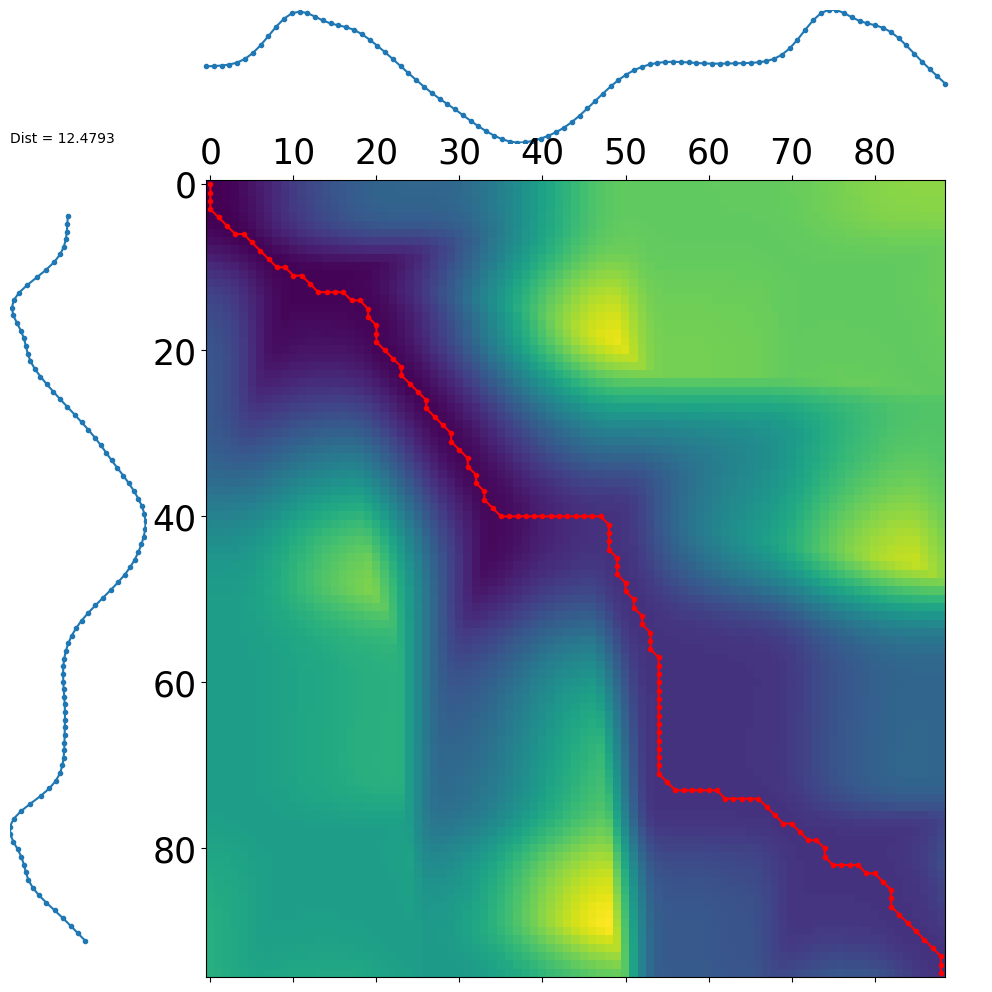
\includegraphics[width=0.99\textwidth]{machine-learning/warping_path_2_curves.png}
    \caption{An illustration of \acrshort{dtw} distance. The big coloured square is the \acrshort{lcm}, each monochromatic subsquare in is an entry in the \acrshort{lcm}. The color of each subsquare indicates the magnitude of the quadratic distance in that entry, blue indicates low, and green and yellow indicate higher values. The red line is the warping path.}
    \label{fig:warping_path}
\end{figure}

TALK ABOUT MAKING DISSIMILARITY MATRIX WITH MULTIVARIATE OBJECTS.

\subsection{Agglomorative Hierarchical Clustering}

The agglomorative hierarchical clustering algorithm is the chosen clustering algorithm in this work. It is a \textit{hard} clustering algorithm meaning that data objects are given a single cluster assignment, and do not have partial memberships to many different clusters. Clustering algorithms that assign data objects partial memberships to many clusters are called \textit{soft} clustering algorithms. \bigskip

\textit{Partional clustering algorithms} is a family of clustering algorithms that are an alternative to the family of hierarchical clustering algorithms. Partional methods work iteratively and rely on defining prototypes that represent the cluster centre. In the first iteration the prototypes are randomly initialized, then the dissimilarity between all data objects and the prototypes are calculated, the data objects are then assigned to the cluster where the dissimilarity to the cluster prototype is minimal. The final step is to update the cluster prototypes such that they best represent the center of the new cluster. These steps repeat untill the value of the cluster prototypes, and cluster membership assignments converge. \bigskip

Hierarchical clustering algorithms have have two central advantages over partitional clustering algorithms, such as K-means, K-medoids and fuzzy C-means. The first advantage is that the user does not have to decide the number of clusters they want to partition the dataset into prior to using the algorithm, the second is that due to the reliance of cluster prototypes, and their random initialization, the cluster assingments yielded when the partitional algorithm are non-deterministic. The clusters assignments that a partitional algorithm converges to is dependent on what values the cluster prototypes are given upon initialization. In fact, CITE ESPEN found that one is not guaranteed convergence at all. Hierarchical clustering algorithms will always yield the same cluster assignments, given that the same dissimilarity matrix is inputed. \bigskip

There are two main types of hierarchical clustering algorithms, \textit{divisive} and \textit{agglomorative}. To understand the difference between these two algorithms, it helps to first understand how agglomorative hierarchical clustering works. Assume one is applying the hierarchical clustering algorithm to cluster a dataset of $N$ data objects. In the initial step, the algorithm takes the dissimilarity matrix as input and every data object in the dataset is regarded as a separate cluster. Next, the case of $N-1$ clusters is considered, two of the existing clusters are merged based on which clusters have the lowest dissimilarity such that there then are $N-1$ clusters. Dissimilarity between clusters is estimated with what is called a \textit{linkage criterion}, that will be expanded upon later. This step of merging existing clusters is repeated until all data objects are contained in one cluster. The result is then a hierarchy of clusters called a \textit{dendrogram}, that can yield cluster assignments at all the possible number of clusters. If one says that agglomorative hierarchical clustering has a bottom-top approach, divisive hierarchical clustering can be said to have a top-bottom approach. It starts at the top of the dendrogram with all data objects in one cluster, and continously splits the cluster until every object is contained in its own cluster. Of the two types of hierarchical clustering the agglomorative approach is the most popular CITATION. What needs to be expanded upon the different types of linkage criterion. In this work seven different linkage criterion are used, which are detailed below.

\begin{itemize}
    \item \textbf{Single linkage}: Computes the dissimilarity between two clusters as the smallest dissimilarity between two individual members of each cluster \cite{dependency_tsc_energy_markets}.
    \item \textbf{Complete linkage}: Computes the dissimilarity between two clusters as the biggest dissimilarity between two individual members of each cluster \cite{financial_tsc_variance_ratio}.
    \item \textbf{Average linkage}: Computes the dissimilarity between two clusters as the average dissimilarity between all members of each cluster \cite{dependency_tsc_energy_markets}.
    \item \textbf{Ward linkage}: Computes the dissimilarity between two clusters as the increase in sum squared dissimilarity of the entire cluster that would be the result of merging the two clusters \cite{copula_ica_tsc}.
    \item \textbf{Centroid linkage}: Computes the dissimilarity between clusters by representing each cluster with a ''centroid'' which is another word for a cluster prototype. Dissimilarity between clusters is then computed as dissimilarity between the centroids of each cluster. After the two clusters are merged a new centroid is computed based on all the cluster members of the two clusters merged. CITE DOCUMENTATION.
    \item \textbf{Median linkage}: Computes dissimilarity between two clusters in the same way as the centroid linkage, the only difference being that after the clusters are merged, the new centroid is computed as the average of the two previous centroids.
    \item \textbf{Weighted linkage}: Works in a method similar to to the average linkage, the only difference being that after two clusters are merged, this linkage requires all the entries in the dissimilarity matrix that pertain to members of this cluster to be averaged. This reduces the number of computations required further down the line because there will be fewer dissimilarity values to average. CITE CODE DOCUMENTATION.
\end{itemize}

SAY SOMETHING ABOUT TIME AND SPACE COMPLEXITY.

\subsection{Curse of Dimensionality}

\section{Deep Neural Networks}

Figure \ref{fig:perc_nn} $(a)$ depicts the building blocks of an ANN, the perceptron. 
The perceptron is a model of an artificial neuron, it takes in $n$ inputs, performs a weighted sum of the inputs and a bias $b$, and sends the sum through an objective function. Originally the objective functions were just threshold functions returning 1 if the sum was above the threshold, and 0 if the sum is below the threshold. When one started using multiple layers of perceptrons as ANNs, other objective functions where introduced including $tanh$, $sigmoid$ and the \textit{recitfied linear unit}. A single perceptron is only able to perform binary classification on points that are linearly separable. However, by combining multiple layers of perceptrons into networks, training the network with the backpropagation algorithm and by intruducing non-linear objective functions ANNs are able to capture complex non-linear relationships. A simple ANN is depicted in figure \ref{fig:perc_nn} $(b)$. The first layer in an ANN is called the input layer, the last layer is called the output layer and all the layers inbetween are called hidden layers. ANNs using special perceptrons with ''memory'' also exist, and are called recurrent neural networks (RNNs). Some ANNs use special layers that only perform wieghted sums with the closest set of neurons from the previous layer, such networks are called convolutional neural networks (CNNs). If one designs an ANN to have as many perceptrons in the output layer as in the input they can be used as a generative model to recreate the input, this is what is known as an autoencoder.

\begin{figure}
\begin{center}
    \tikzstyle{init} = [pin edge={to-,thin,black}]
\tikzstyle{circ} = [circle, minimum size=1cm, text centered, draw=black, fill=blue!20]
\tikzstyle{arrow} = [thin,->,>=stealth]
\tikzstyle{arrow_t} = [very thin,->,>=stealth]

\tikzstyle{perc_in} = [circle, minimum size=1mm, text centered, draw=black, fill=blue!20]
\tikzstyle{perc_ou} = [circle, minimum size=1mm, text centered, draw=black, fill=red!20]
\tikzstyle{perc_hi} = [circle, minimum size=1mm, text centered, draw=black, fill=green!20]

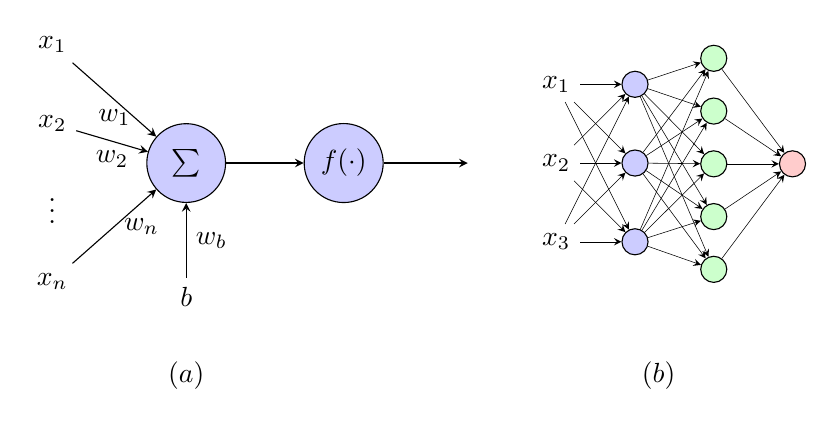
\begin{tikzpicture}
% Perceptron
\node (x1) [init] {$x_1$};
\node (x2) [init, below of=x1] {$x_2$};
\node (vdots) [init, below of=x2] {$\vdots$};
\node (xn) [init, below of=vdots] {$x_n$};

\node (sum) [circ, right of=x2, xshift=0.7cm, yshift=-5mm] {$\sum$};
\node (b) [init, below of=sum, yshift=-0.7cm] {$b$};
\node (obj) [circ, right of=sum, xshift=1cm] {$f(\cdot)$};
\node (output) [init, right of=obj, xshift=0.7cm] {};

\draw [arrow] (x1) --node[anchor=north] {$w_1$} (sum);
\draw [arrow] (x2) --node[anchor=north] {$w_2$} (sum);
\draw [arrow] (xn) --node[anchor=west] {$w_n$} (sum);
\draw [arrow] (b) --node[anchor=west] {$w_b$} (sum);
\draw [arrow] (sum) -- (obj);
\draw [arrow] (obj) -- (output);

% ANN
\node (i2) [init, right of=output] {$x_2$};
\node (i1) [init,, above of=i2] {$x_1$};
\node (i3) [init, below of=i2] {$x_3$};

\node (in0) [perc_in, right of=i1] {};
\node (in1) [perc_in, below of=in0] {};
\node (in2) [perc_in, below of=in1] {};

\node (hi0) [perc_hi, right of=in0, yshift=3.3mm] {};
\node (hi1) [perc_hi, below of=hi0, yshift=3.3mm] {};
\node (hi2) [perc_hi, below of=hi1, yshift=3.3mm] {};
\node (hi3) [perc_hi, below of=hi2, yshift=3.3mm] {};
\node (hi4) [perc_hi, below of=hi3, yshift=3.3mm] {};

\node (ou0) [perc_ou, right of=hi2] {};

\draw [arrow_t] (i1) -- (in0);
\draw [arrow_t] (i1) -- (in1);
\draw [arrow_t] (i1) -- (in2);
\draw [arrow_t] (i2) -- (in0);
\draw [arrow_t] (i2) -- (in1);
\draw [arrow_t] (i2) -- (in2);
\draw [arrow_t] (i3) -- (in0);
\draw [arrow_t] (i3) -- (in1);
\draw [arrow_t] (i3) -- (in2);

\draw [arrow_t] (in0) -- (hi0);
\draw [arrow_t] (in0) -- (hi1);
\draw [arrow_t] (in0) -- (hi2);
\draw [arrow_t] (in0) -- (hi3);
\draw [arrow_t] (in0) -- (hi4);
\draw [arrow_t] (in1) -- (hi0);
\draw [arrow_t] (in1) -- (hi1);
\draw [arrow_t] (in1) -- (hi2);
\draw [arrow_t] (in1) -- (hi3);
\draw [arrow_t] (in1) -- (hi4);
\draw [arrow_t] (in2) -- (hi0);
\draw [arrow_t] (in2) -- (hi1);
\draw [arrow_t] (in2) -- (hi2);
\draw [arrow_t] (in2) -- (hi3);
\draw [arrow_t] (in2) -- (hi4);

\draw [arrow_t] (hi0) -- (ou0);
\draw [arrow_t] (hi1) -- (ou0);
\draw [arrow_t] (hi2) -- (ou0);
\draw [arrow_t] (hi3) -- (ou0);
\draw [arrow_t] (hi4) -- (ou0);

\node (label_a) [init, below of=b] {$(a)$};
\node (label_a) [init, right of=label_a, xshift=5cm] {$(b)$};
\end{tikzpicture}
\end{center}
\caption{$(a)$ A Perceptron. $(b)$ Example of a simple ANN.} 
\label{fig:perc_nn}
\end{figure}

\subsection{Multi-layer Perceptrons and Objective Functions}

\subsection{Training}

\subsection{Convolutional Layers}

\subsection{Recurrent Layers}

\subsection{Overfitting}
 
